\subsection{Decision 8: Interaction with ticket scanners}

\subsection*{Status}
Open
\subsection*{Architectural Summary}


\subsection*{Concern}
Passengers want a seamless travel experience, without being mistakenly blocked at the turnstiles.
Tycoons want to admit only paying passengers in trains, avoiding controllers costs.
Turnstiles need to communicate with the system to ensure correct and quick verification of the requisites to be allowed in the station.

\subsubsection*{User Stories}
The decision on how turnstiles interact with the payment system is integral to ensuring a seamless travel experience and securing access to train areas. Below, we detail specific user stories connected to this architectural decision, highlighting the requirements and expectations from various stakeholders.

\begin{enumerate}[noitemsep]
    \item \textbf{User Story 1 (Frequent Traveler's Monthly Pass)}: A comprehensive monthly pass needs to be recognized by the turnstiles, necessitating a system that supports seamless access for subscribers.
    
    \item \textbf{User Story 2 (Online Balance Check for Multi-Network Travel Card)}: The system requires turnstiles to accurately read and verify travel card balances to prevent entry issues, emphasizing the need for an integrated payment system.
    
    \item \textbf{User Story 15 (Prevention of Payment for Temporarily Blocked Routes)}: This story underscores the importance of turnstiles having up-to-date information on route availability to avoid mistakenly blocking passengers.
    
    \item \textbf{User Story 16 (Single Ticket for All Train Networks)}: Turnstiles must effectively communicate with the payment system to recognize and approve tickets valid across different networks, ensuring seamless travel.
    
    \item \textbf{User Story 26 (Real-time Updates for Station Managers)}: The technology supporting real-time updates can also enhance turnstile interactions, ensuring entry permissions reflect current ticketing information based on schedules and disruptions.
    
    \item \textbf{User Story 27 (Integration with Maintenance Scheduling)}: Turnstiles must adapt to maintenance schedules, allowing for adjustments in access permissions, which suggests the need for a flexible and responsive payment system.
    
    \item \textbf{User Story 23 (Payment System Integration for Tycoons)}: The story relates to the seamless integration of turnstiles with updated payment systems, crucial for maintaining high service levels and secure access.
\end{enumerate}

These user stories collectively highlight the diverse requirements for the turnstile and payment system interaction, from seamless access and real-time information integration to flexibility in handling various ticketing formats and system updates.
The problem can be made more abstract, as the interaction with the turnstile can be similar to the following interactions:
\begin{itemize}
    \item interaction with a controller who scans the ticket or any proof of subscription.
    \item interaction with a scanner onboard a bus.
\end{itemize}

\subsection*{Context}

Most stations, expecially the big ones, have turnstiles to avoid people without tickets to enter the trains area.
The turnstiles should communicate with the system to ensure this. A decision should be taken on who to admit in the station.
This logic could be provided by the station manager or by the tycoons, or even by TrIP managment.
How do the passenger input its ticket or subscription or prepaid card to the turnstile?
How does the turnstile communicate with the system to verify if the passenger has the right to enter the station?

\subsection*{Criteria}
\begin{itemize}
    \item Allow users to scan tickets or multiplatform travel cards (if they exists) at turnstiles.
    \item Don't allow people without the appropriate tickets or subscriptions or cards.
    \item Possibly allow people to scan when they enter and when they exit and calculate a fare (this might depend on agreements between tycoons). 
    \item Possibly communicate station usage data to the system.
    \item Possibly allow credit/debit card scan.
    \item Allow balance check for charged cards.
\end{itemize}

\subsection*{Option 1: Add a ticket checker and a user state modules to authorize user}
After scanning a ticket or badge, the user state should be updated, in order to calculate the fare price for fillable card holders or for the scanning of bank cards (debit credit).
The ticket or badge should be checked by the single ticket checker module or by the account management to insure consistency.
In case of the scanning of bank cards, the user state module needs to communicate with payment management, in order to proceed with the actual payment.
The scanning of bank cards and fillable cards create the needs for a calculation of appropriate revenue share between different tycoon. This should be the topic of a future decision or might be incorporated in this one.
\begin{figure}[ht]
    \centering
    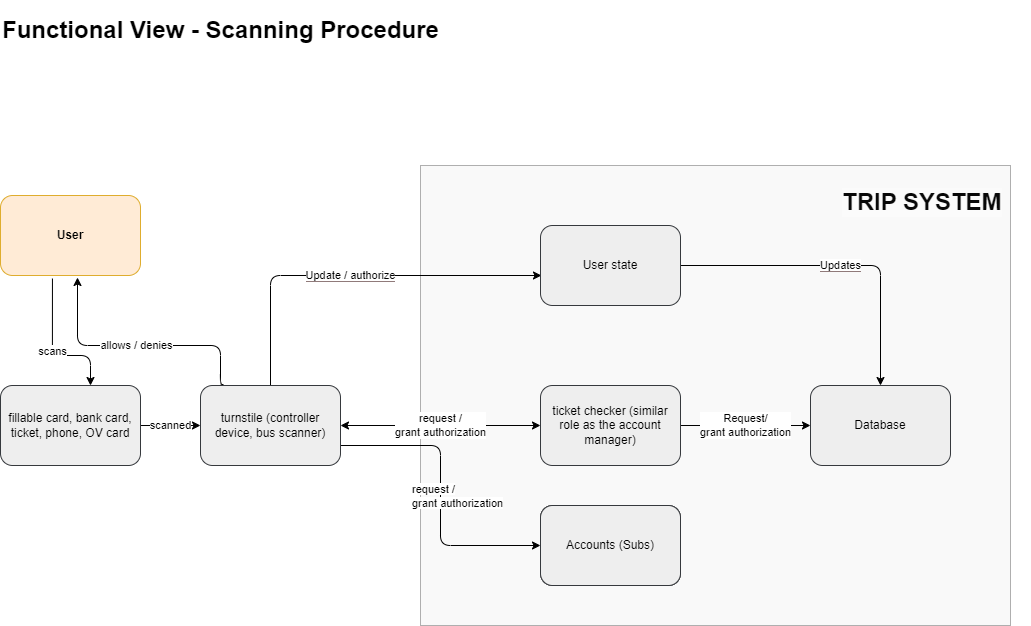
\includegraphics[width=\textwidth]{drawings/views_draft2/functional_view turnstiles.png}
    \caption{Interaction with a ticket scanner.}
    \label{fig:ticket_scanner}
\end{figure}

\subsection*{Option 2: Allow fillable cards, account cards and tickets, not bank cards}
Not allowing bank cards at turnstiles simplifies the job of turnstiles.
Also, how can a controller check if the traveller have scanned a bank card when entering the turnstile?
We can have the turnstile print a ticket with a barcode or QR code.


\subsection*{Decision}

\subsection*{Consequences}
\textbf{Positive Consequences:}
% \begin{itemize}
% \end{itemize}
\textbf{Negative Consequences:}
% \begin{itemize}
% \end{itemize}